
\usepackage{amssymb}
\usepackage{tikz}
\usetikzlibrary{calc}
\usetikzlibrary{chains}
\usetikzlibrary{scopes}
\usetikzlibrary{shapes.geometric}
\usetikzlibrary{trees}
\usetikzlibrary{topaths}
\usetikzlibrary{positioning}
\usetikzlibrary{patterns,decorations.pathreplacing}

\newcommand{\bP}{\mathbb P}

\newcommand{\Pst}{{\mathbb P}\left(
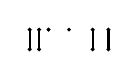
\begin{tikzpicture}[baseline=1pt]
 \draw [fill] (0,0) circle(0.12ex);
 \draw [fill] (0.12,0) circle(0.12ex);
 \draw [fill] (0,0.25) circle(0.12ex);
 \draw [fill] (0.12,0.25) circle(0.12ex);
 \draw [fill] (1,0) circle(0.12ex);
 \draw [fill] (0.8,0) circle(0.12ex);
 \draw [fill] (1,0.25) circle(0.12ex);
 \draw [fill] (0.8,0.25) circle(0.12ex);
  \draw [thick] (0,0)--(0,0.25);
 \draw [thick] (0.12,0)--(0.12,0.25);
  \draw [thick] (0.8,0)--(0.8,0.25);
 \draw [thick] (1,0)--(1,0.25);
  \draw [fill] (0.24,0.25) circle(0.1ex);
 \draw [fill] (0.5,0.25) circle(0.1ex);
 \draw [fill] (0.24,0.25) circle(0.1ex);
 \end{tikzpicture}
\right)}

\newcommand{\Pnn}{{\mathbb P}\left(
\begin{tikzpicture}[baseline=1pt]
 \draw [fill] (0,0) circle(0.12ex);
 \draw [fill] (0.12,0) circle(0.12ex);
 \draw [fill] (0,0.25) circle(0.12ex);
 \draw [fill] (0.12,0.25) circle(0.12ex);
 \end{tikzpicture}
\right)}

%%%
\newcommand{\PAa}{{\mathbb P}\left(
\begin{tikzpicture}[baseline=1pt]
 \draw [fill] (0,0) circle(0.12ex);
 \draw [fill] (0.12,0) circle(0.12ex);
 \draw [fill] (0,0.25) circle(0.12ex);
 \draw [fill] (0.12,0.25) circle(0.12ex);
 \draw [thick] (0,0)--(0,0.25);
 % \draw [thick] (0.12,0)--(0.12,0.25);
 \end{tikzpicture}
\right)}

\newcommand{\PBb}{{\mathbb P}\left(
\begin{tikzpicture}[baseline=1pt]
 \draw [fill] (0,0) circle(0.12ex);
 \draw [fill] (0.12,0) circle(0.12ex);
 \draw [fill] (0,0.25) circle(0.12ex);
 \draw [fill] (0.12,0.25) circle(0.12ex);
 % \draw [thick] (0,0)--(0,0.25);
 \draw [thick] (0.12,0)--(0.12,0.25);
 \end{tikzpicture}
\right)}

\newcommand{\PAb}{{\mathbb P}\left(
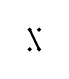
\begin{tikzpicture}[baseline=1pt]
 \draw [fill] (0,0) circle(0.12ex);
 \draw [fill] (0.12,0) circle(0.12ex);
 \draw [fill] (0,0.25) circle(0.12ex);
 \draw [fill] (0.12,0.25) circle(0.12ex);
 % \draw [thick] (0,0)--(0.12,0.25);
 \draw [thick] (0.12,0)--(0.,0.25);
 \end{tikzpicture}
\right)}

\newcommand{\PBa}{{\mathbb P}\left(
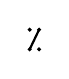
\begin{tikzpicture}[baseline=1pt]
 \draw [fill] (0,0) circle(0.12ex);
 \draw [fill] (0.12,0) circle(0.12ex);
 \draw [fill] (0,0.25) circle(0.12ex);
 \draw [fill] (0.12,0.25) circle(0.12ex);
 \draw [thick] (0,0)--(0.12,0.25);
 % \draw [thick] (0.12,0)--(0.,0.25);
 \end{tikzpicture}
\right)}


%%%%



\newcommand{\Ps}{{\mathbb P}\left(
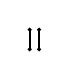
\begin{tikzpicture}[baseline=1pt]
 \draw [fill] (0,0) circle(0.12ex);
 \draw [fill] (0.12,0) circle(0.12ex);
 \draw [fill] (0,0.25) circle(0.12ex);
 \draw [fill] (0.12,0.25) circle(0.12ex);
 \draw [thick] (0,0)--(0,0.25);
 \draw [thick] (0.12,0)--(0.12,0.25);
 \end{tikzpicture}
\right)}

\newcommand{\Pc}{{\mathbb P}\left(
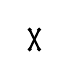
\begin{tikzpicture}[baseline=1pt]
 \draw [fill] (0,0) circle(0.12ex);
 \draw [fill] (0.12,0) circle(0.12ex);
 \draw [fill] (0,0.25) circle(0.12ex);
 \draw [fill] (0.12,0.25) circle(0.12ex);
 \draw [thick] (0,0)--(0.12,0.25);
 \draw [thick] (0.12,0)--(0.,0.25);
 \end{tikzpicture}
\right)}

\newcommand{\Panan}{{\mathbb P}\left(
\begin{tikzpicture}[baseline=1pt]
 \draw [fill] (0,0) circle(0.12ex);
 \draw [fill] (0.12,0) circle(0.12ex);
 \draw [fill] (0,0.25) circle(0.12ex);
 \draw [fill] (0.12,0.25) circle(0.12ex);
 \draw [thick] (0,0)--(0,0.25);
 \end{tikzpicture}
\right)}

\newcommand{\Pnbnb}{{\mathbb P}\left(
\begin{tikzpicture}[baseline=1pt]
 \draw [fill] (0,0) circle(0.12ex);
 \draw [fill] (0.12,0) circle(0.12ex);
 \draw [fill] (0,0.25) circle(0.12ex);
 \draw [fill] (0.12,0.25) circle(0.12ex);
 \draw [thick] (0.12,0)--(0.12,0.25);
 \end{tikzpicture}
\right)}

\newcommand{\Pannb}{{\mathbb P}\left(
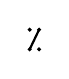
\begin{tikzpicture}[baseline=1pt]
 \draw [fill] (0,0) circle(0.12ex);
 \draw [fill] (0.12,0) circle(0.12ex);
 \draw [fill] (0,0.25) circle(0.12ex);
 \draw [fill] (0.12,0.25) circle(0.12ex);
 \draw [thick] (0,0)--(0.12,0.25);
 \end{tikzpicture}
\right)}

\newcommand{\Pnban}{{\mathbb P}\left(
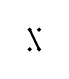
\begin{tikzpicture}[baseline=1pt]
 \draw [fill] (0,0) circle(0.12ex);
 \draw [fill] (0.12,0) circle(0.12ex);
 \draw [fill] (0,0.25) circle(0.12ex);
 \draw [fill] (0.12,0.25) circle(0.12ex);
 \draw [thick] (0.12,0)--(0.,0.25);
 \end{tikzpicture}
\right)}

\newcommand{\Pabc}{{\mathbb P}\left(
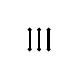
\begin{tikzpicture}[baseline=1pt]
 \draw [fill] (0,0) circle(0.12ex);
 \draw [fill] (0.12,0) circle(0.12ex);
 \draw [fill] (0,0.25) circle(0.12ex);
 \draw [fill] (0.12,0.25) circle(0.12ex);
  \draw [fill] (0.24,0.) circle(0.12ex);
 \draw [fill] (0.24,0.25) circle(0.12ex);
 \draw [thick] (0,0)--(0,0.25);
 \draw [thick] (0.12,0)--(0.12,0.25);
  \draw [thick] (0.24,0)--(0.24,0.25);
 \end{tikzpicture}
\right)}

\newcommand{\Pbac}{{\mathbb P}\left(
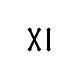
\begin{tikzpicture}[baseline=1pt]
 \draw [fill] (0,0) circle(0.12ex);
 \draw [fill] (0.12,0) circle(0.12ex);
 \draw [fill] (0,0.25) circle(0.12ex);
 \draw [fill] (0.12,0.25) circle(0.12ex);
  \draw [fill] (0.24,0.25) circle(0.12ex);
   \draw [fill] (0.24,0) circle(0.12ex);
 \draw [thick] (0,0)--(0.12,0.25);
 \draw [thick] (0.12,0)--(0.,0.25);
  \draw [thick] (0.24,0)--(0.24,0.25);
 \end{tikzpicture}
\right)}

\newcommand{\Pacb}{{\mathbb P}\left(
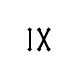
\begin{tikzpicture}[baseline=1pt]
 \draw [fill] (0,0) circle(0.12ex);
 \draw [fill] (0.12,0) circle(0.12ex);
 \draw [fill] (0,0.25) circle(0.12ex);
 \draw [fill] (0.12,0.25) circle(0.12ex);
  \draw [fill] (0.24,0.25) circle(0.12ex);
   \draw [fill] (0.24,0) circle(0.12ex);
 \draw [thick] (0.12,0)--(0.24,0.25);
 \draw [thick] (0.24,0)--(0.12,0.25);
  \draw [thick] (0.,0)--(0.,0.25);
 \end{tikzpicture}
\right)}

\newcommand{\Pcba}{{\mathbb P}\left(

\begin{tikzpicture}[baseline=1pt]
 \draw [fill] (0,0) circle(0.12ex);
 \draw [fill] (0.12,0) circle(0.12ex);
 \draw [fill] (0,0.25) circle(0.12ex);
 \draw [fill] (0.12,0.25) circle(0.12ex);
  \draw [fill] (0.24,0.25) circle(0.12ex);
   \draw [fill] (0.24,0) circle(0.12ex);
 \draw [thick] (0.,0)--(0.24,0.25);
 \draw [thick] (0.24,0)--(0.,0.25);
  \draw [thick] (0.12,0)--(0.12,0.25);
 \end{tikzpicture}
\right)}

\newcommand{\Pbca}{{\mathbb P}\left(

\begin{tikzpicture}[baseline=1pt]
 \draw [fill] (0,0) circle(0.12ex);
 \draw [fill] (0.12,0) circle(0.12ex);
 \draw [fill] (0,0.25) circle(0.12ex);
 \draw [fill] (0.12,0.25) circle(0.12ex);
  \draw [fill] (0.24,0.25) circle(0.12ex);
   \draw [fill] (0.24,0) circle(0.12ex);
 \draw [thick] (0.,0)--(0.12,0.25);
  \draw [thick] (0.12,0.)--(0.24,0.25);
 \draw [thick] (0.24,0)--(0.,0.25);
 \end{tikzpicture}
\right)}

\newcommand{\Pcab}{{\mathbb P}\left(

\begin{tikzpicture}[baseline=1pt]
 \draw [fill] (0,0) circle(0.12ex);
 \draw [fill] (0.12,0) circle(0.12ex);
 \draw [fill] (0,0.25) circle(0.12ex);
 \draw [fill] (0.12,0.25) circle(0.12ex);
  \draw [fill] (0.24,0.25) circle(0.12ex);
   \draw [fill] (0.24,0) circle(0.12ex);
 \draw [thick] (0.,0)--(0.24,0.25);
  \draw [thick] (0.12,0.)--(0.,0.25);
 \draw [thick] (0.24,0)--(0.12,0.25);
 \end{tikzpicture}
\right)}

\newcommand{\Pex}{{\mathbb P}\left(
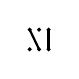
\begin{tikzpicture}[baseline=1pt]
 \draw [fill] (0,0) circle(0.12ex);
 \draw [fill] (0.12,0) circle(0.12ex);
 \draw [fill] (0,0.25) circle(0.12ex);
 \draw [fill] (0.12,0.25) circle(0.12ex);
  \draw [fill] (0.24,0.25) circle(0.12ex);
   \draw [fill] (0.24,0) circle(0.12ex);
  \draw [thick] (0.12,0.)--(0.,0.25);
 \draw [thick] (0.24,0)--(0.24,0.25);
 \end{tikzpicture}
\right)}

\newcommand{\Pabn}{{\mathbb P}\left(
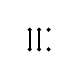
\begin{tikzpicture}[baseline=1pt]
 \draw [fill] (0,0) circle(0.12ex);
 \draw [fill] (0.12,0) circle(0.12ex);
 \draw [fill] (0,0.25) circle(0.12ex);
 \draw [fill] (0.12,0.25) circle(0.12ex);
  \draw [fill] (0.24,0.25) circle(0.12ex);
   \draw [fill] (0.24,0) circle(0.12ex);
 \draw [thick] (0.,0)--(0.,0.25);
  \draw [thick] (0.12,0.)--(0.12,0.25);
 \end{tikzpicture}
\right)}

\newcommand{\Pabnabn}{{\mathbb P}\left(
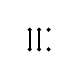
\begin{tikzpicture}[baseline=1pt]
 \draw [fill] (0,0) circle(0.12ex);
 \draw [fill] (0.12,0) circle(0.12ex);
 \draw [fill] (0,0.25) circle(0.12ex);
 \draw [fill] (0.12,0.25) circle(0.12ex);
  \draw [fill] (0.24,0.25) circle(0.12ex);
   \draw [fill] (0.24,0) circle(0.12ex);
 \draw [thick] (0.,0)--(0.,0.25);
  \draw [thick] (0.12,0.)--(0.12,0.25);
 \end{tikzpicture}
\right)}

\newcommand{\Pabnanb}{{\mathbb P}\left(
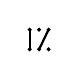
\begin{tikzpicture}[baseline=1pt]
 \draw [fill] (0,0) circle(0.12ex);
 \draw [fill] (0.12,0) circle(0.12ex);
 \draw [fill] (0,0.25) circle(0.12ex);
 \draw [fill] (0.12,0.25) circle(0.12ex);
  \draw [fill] (0.24,0.25) circle(0.12ex);
   \draw [fill] (0.24,0) circle(0.12ex);
 \draw [thick] (0.,0)--(0.,0.25);
  \draw [thick] (0.12,0.)--(0.24,0.25);
 \end{tikzpicture}
\right)}

\newcommand{\Pabnnab}{{\mathbb P}\left(
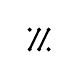
\begin{tikzpicture}[baseline=1pt]
 \draw [fill] (0,0) circle(0.12ex);
 \draw [fill] (0.12,0) circle(0.12ex);
 \draw [fill] (0,0.25) circle(0.12ex);
 \draw [fill] (0.12,0.25) circle(0.12ex);
  \draw [fill] (0.24,0.25) circle(0.12ex);
   \draw [fill] (0.24,0) circle(0.12ex);
 \draw [thick] (0.,0)--(0.12,0.25);
  \draw [thick] (0.12,0.)--(0.24,0.25);
 \end{tikzpicture}
\right)}

\newcommand{\Pabnban}{{\mathbb P}\left(
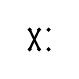
\begin{tikzpicture}[baseline=1pt]
 \draw [fill] (0,0) circle(0.12ex);
 \draw [fill] (0.12,0) circle(0.12ex);
 \draw [fill] (0,0.25) circle(0.12ex);
 \draw [fill] (0.12,0.25) circle(0.12ex);
  \draw [fill] (0.24,0.25) circle(0.12ex);
   \draw [fill] (0.24,0) circle(0.12ex);
 \draw [thick] (0.,0)--(0.12,0.25);
  \draw [thick] (0.12,0.)--(0.,0.25);
 \end{tikzpicture}
\right)}

\newcommand{\Pabnbna}{{\mathbb P}\left(
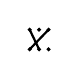
\begin{tikzpicture}[baseline=1pt]
 \draw [fill] (0,0) circle(0.12ex);
 \draw [fill] (0.12,0) circle(0.12ex);
 \draw [fill] (0,0.25) circle(0.12ex);
 \draw [fill] (0.12,0.25) circle(0.12ex);
  \draw [fill] (0.24,0.25) circle(0.12ex);
   \draw [fill] (0.24,0) circle(0.12ex);
 \draw [thick] (0.,0)--(0.24,0.25);
  \draw [thick] (0.12,0.)--(0.,0.25);
 \end{tikzpicture}
\right)}

\newcommand{\Pabnnba}{{\mathbb P}\left(
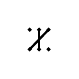
\begin{tikzpicture}[baseline=1pt]
 \draw [fill] (0,0) circle(0.12ex);
 \draw [fill] (0.12,0) circle(0.12ex);
 \draw [fill] (0,0.25) circle(0.12ex);
 \draw [fill] (0.12,0.25) circle(0.12ex);
  \draw [fill] (0.24,0.25) circle(0.12ex);
   \draw [fill] (0.24,0) circle(0.12ex);
 \draw [thick] (0.,0)--(0.24,0.25);
  \draw [thick] (0.12,0.)--(0.12,0.25);
 \end{tikzpicture}
\right)}



\newcommand{\Panbabn}{{\mathbb P}\left(
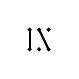
\begin{tikzpicture}[baseline=1pt]
 \draw [fill] (0,0) circle(0.12ex);
 \draw [fill] (0.12,0) circle(0.12ex);
 \draw [fill] (0,0.25) circle(0.12ex);
 \draw [fill] (0.12,0.25) circle(0.12ex);
  \draw [fill] (0.24,0.25) circle(0.12ex);
   \draw [fill] (0.24,0) circle(0.12ex);
 \draw [thick] (0.,0)--(0.,0.25);
  \draw [thick] (0.24,0.)--(0.12,0.25);
 \end{tikzpicture}
\right)}

\newcommand{\Panbanb}{{\mathbb P}\left(
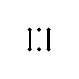
\begin{tikzpicture}[baseline=1pt]
 \draw [fill] (0,0) circle(0.12ex);
 \draw [fill] (0.12,0) circle(0.12ex);
 \draw [fill] (0,0.25) circle(0.12ex);
 \draw [fill] (0.12,0.25) circle(0.12ex);
  \draw [fill] (0.24,0.25) circle(0.12ex);
   \draw [fill] (0.24,0) circle(0.12ex);
 \draw [thick] (0.,0)--(0.,0.25);
\draw [thick] (0.24,0.)--(0.24,0.25);
 \end{tikzpicture}
\right)}

\newcommand{\Panbnab}{{\mathbb P}\left(
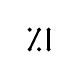
\begin{tikzpicture}[baseline=1pt]
 \draw [fill] (0,0) circle(0.12ex);
 \draw [fill] (0.12,0) circle(0.12ex);
 \draw [fill] (0,0.25) circle(0.12ex);
 \draw [fill] (0.12,0.25) circle(0.12ex);
  \draw [fill] (0.24,0.25) circle(0.12ex);
   \draw [fill] (0.24,0) circle(0.12ex);
 \draw [thick] (0.,0)--(0.12,0.25);
\draw [thick] (0.24,0.)--(0.24,0.25);
 \end{tikzpicture}
\right)}

\newcommand{\Panbban}{{\mathbb P}\left(
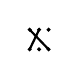
\begin{tikzpicture}[baseline=1pt]
 \draw [fill] (0,0) circle(0.12ex);
 \draw [fill] (0.12,0) circle(0.12ex);
 \draw [fill] (0,0.25) circle(0.12ex);
 \draw [fill] (0.12,0.25) circle(0.12ex);
  \draw [fill] (0.24,0.25) circle(0.12ex);
   \draw [fill] (0.24,0) circle(0.12ex);
 \draw [thick] (0.,0)--(0.12,0.25);
\draw [thick] (0.24,0.)--(0.,0.25);
 \end{tikzpicture}
\right)}

\newcommand{\Panbbna}{{\mathbb P}\left(

\begin{tikzpicture}[baseline=1pt]
 \draw [fill] (0,0) circle(0.12ex);
 \draw [fill] (0.12,0) circle(0.12ex);
 \draw [fill] (0,0.25) circle(0.12ex);
 \draw [fill] (0.12,0.25) circle(0.12ex);
  \draw [fill] (0.24,0.25) circle(0.12ex);
   \draw [fill] (0.24,0) circle(0.12ex);
 \draw [thick] (0.,0)--(0.24,0.25);
\draw [thick] (0.24,0.)--(0.,0.25);
 \end{tikzpicture}
\right)}

\newcommand{\Panbnba}{{\mathbb P}\left(
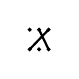
\begin{tikzpicture}[baseline=1pt]
 \draw [fill] (0,0) circle(0.12ex);
 \draw [fill] (0.12,0) circle(0.12ex);
 \draw [fill] (0,0.25) circle(0.12ex);
 \draw [fill] (0.12,0.25) circle(0.12ex);
  \draw [fill] (0.24,0.25) circle(0.12ex);
   \draw [fill] (0.24,0) circle(0.12ex);
 \draw [thick] (0.,0)--(0.24,0.25);
\draw [thick] (0.24,0.)--(0.12,0.25);
 \end{tikzpicture}
\right)}

\newcommand{\Pnababn}{{\mathbb P}\left(
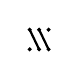
\begin{tikzpicture}[baseline=1pt]
 \draw [fill] (0,0) circle(0.12ex);
 \draw [fill] (0.12,0) circle(0.12ex);
 \draw [fill] (0,0.25) circle(0.12ex);
 \draw [fill] (0.12,0.25) circle(0.12ex);
  \draw [fill] (0.24,0.25) circle(0.12ex);
   \draw [fill] (0.24,0) circle(0.12ex);
 \draw [thick] (0.12,0)--(0.,0.25);
  \draw [thick] (0.24,0.)--(0.12,0.25);
 \end{tikzpicture}
\right)}

\newcommand{\Pnabanb}{{\mathbb P}\left(
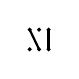
\begin{tikzpicture}[baseline=1pt]
 \draw [fill] (0,0) circle(0.12ex);
 \draw [fill] (0.12,0) circle(0.12ex);
 \draw [fill] (0,0.25) circle(0.12ex);
 \draw [fill] (0.12,0.25) circle(0.12ex);
  \draw [fill] (0.24,0.25) circle(0.12ex);
   \draw [fill] (0.24,0) circle(0.12ex);
 \draw [thick] (0.12,0)--(0.,0.25);
\draw [thick] (0.24,0.)--(0.24,0.25);
 \end{tikzpicture}
\right)}

\newcommand{\Pnabnab}{{\mathbb P}\left(
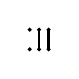
\begin{tikzpicture}[baseline=1pt]
 \draw [fill] (0,0) circle(0.12ex);
 \draw [fill] (0.12,0) circle(0.12ex);
 \draw [fill] (0,0.25) circle(0.12ex);
 \draw [fill] (0.12,0.25) circle(0.12ex);
  \draw [fill] (0.24,0.25) circle(0.12ex);
   \draw [fill] (0.24,0) circle(0.12ex);
 \draw [thick] (0.12,0)--(0.12,0.25);
\draw [thick] (0.24,0.)--(0.24,0.25);
 \end{tikzpicture}
\right)}

\newcommand{\Pnabban}{{\mathbb P}\left(
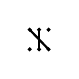
\begin{tikzpicture}[baseline=1pt]
 \draw [fill] (0,0) circle(0.12ex);
 \draw [fill] (0.12,0) circle(0.12ex);
 \draw [fill] (0,0.25) circle(0.12ex);
 \draw [fill] (0.12,0.25) circle(0.12ex);
  \draw [fill] (0.24,0.25) circle(0.12ex);
   \draw [fill] (0.24,0) circle(0.12ex);
 \draw [thick] (0.12,0)--(0.12,0.25);
\draw [thick] (0.24,0.)--(0.,0.25);
 \end{tikzpicture}
\right)}

\newcommand{\Pnabbna}{{\mathbb P}\left(
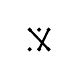
\begin{tikzpicture}[baseline=1pt]
 \draw [fill] (0,0) circle(0.12ex);
 \draw [fill] (0.12,0) circle(0.12ex);
 \draw [fill] (0,0.25) circle(0.12ex);
 \draw [fill] (0.12,0.25) circle(0.12ex);
  \draw [fill] (0.24,0.25) circle(0.12ex);
   \draw [fill] (0.24,0) circle(0.12ex);
 \draw [thick] (0.12,0)--(0.24,0.25);
\draw [thick] (0.24,0.)--(0.,0.25);
 \end{tikzpicture}
\right)}

\newcommand{\Pnabnba}{{\mathbb P}\left(
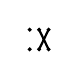
\begin{tikzpicture}[baseline=1pt]
 \draw [fill] (0,0) circle(0.12ex);
 \draw [fill] (0.12,0) circle(0.12ex);
 \draw [fill] (0,0.25) circle(0.12ex);
 \draw [fill] (0.12,0.25) circle(0.12ex);
  \draw [fill] (0.24,0.25) circle(0.12ex);
   \draw [fill] (0.24,0) circle(0.12ex);
 \draw [thick] (0.12,0)--(0.24,0.25);
\draw [thick] (0.24,0.)--(0.12,0.25);
 \end{tikzpicture}
\right)}




\newcommand{\Pannann}{{\mathbb P}\left(
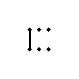
\begin{tikzpicture}[baseline=1pt]
 \draw [fill] (0,0) circle(0.12ex);
 \draw [fill] (0.12,0) circle(0.12ex);
 \draw [fill] (0,0.25) circle(0.12ex);
 \draw [fill] (0.12,0.25) circle(0.12ex);
  \draw [fill] (0.24,0.25) circle(0.12ex);
   \draw [fill] (0.24,0) circle(0.12ex);
 \draw [thick] (0.,0)--(0.,0.25);
 \end{tikzpicture}
\right)}

\newcommand{\Pannnan}{{\mathbb P}\left(
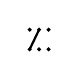
\begin{tikzpicture}[baseline=1pt]
 \draw [fill] (0,0) circle(0.12ex);
 \draw [fill] (0.12,0) circle(0.12ex);
 \draw [fill] (0,0.25) circle(0.12ex);
 \draw [fill] (0.12,0.25) circle(0.12ex);
  \draw [fill] (0.24,0.25) circle(0.12ex);
   \draw [fill] (0.24,0) circle(0.12ex);
 \draw [thick] (0.,0)--(0.12,0.25);
 \end{tikzpicture}
\right)}

\newcommand{\Pannnna}{{\mathbb P}\left(
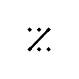
\begin{tikzpicture}[baseline=1pt]
 \draw [fill] (0,0) circle(0.12ex);
 \draw [fill] (0.12,0) circle(0.12ex);
 \draw [fill] (0,0.25) circle(0.12ex);
 \draw [fill] (0.12,0.25) circle(0.12ex);
  \draw [fill] (0.24,0.25) circle(0.12ex);
   \draw [fill] (0.24,0) circle(0.12ex);
 \draw [thick] (0.,0)--(0.24,0.25);
 \end{tikzpicture}
\right)}

\newcommand{\Pnanann}{{\mathbb P}\left(
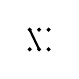
\begin{tikzpicture}[baseline=1pt]
 \draw [fill] (0,0) circle(0.12ex);
 \draw [fill] (0.12,0) circle(0.12ex);
 \draw [fill] (0,0.25) circle(0.12ex);
 \draw [fill] (0.12,0.25) circle(0.12ex);
  \draw [fill] (0.24,0.25) circle(0.12ex);
   \draw [fill] (0.24,0) circle(0.12ex);
 \draw [thick] (0.12,0)--(0.,0.25);
 \end{tikzpicture}
\right)}

\newcommand{\Pnannan}{{\mathbb P}\left(
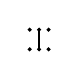
\begin{tikzpicture}[baseline=1pt]
 \draw [fill] (0,0) circle(0.12ex);
 \draw [fill] (0.12,0) circle(0.12ex);
 \draw [fill] (0,0.25) circle(0.12ex);
 \draw [fill] (0.12,0.25) circle(0.12ex);
  \draw [fill] (0.24,0.25) circle(0.12ex);
   \draw [fill] (0.24,0) circle(0.12ex);
 \draw [thick] (0.12,0)--(0.12,0.25);
 \end{tikzpicture}
\right)}

\newcommand{\Pnannna}{{\mathbb P}\left(
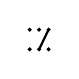
\begin{tikzpicture}[baseline=1pt]
 \draw [fill] (0,0) circle(0.12ex);
 \draw [fill] (0.12,0) circle(0.12ex);
 \draw [fill] (0,0.25) circle(0.12ex);
 \draw [fill] (0.12,0.25) circle(0.12ex);
  \draw [fill] (0.24,0.25) circle(0.12ex);
   \draw [fill] (0.24,0) circle(0.12ex);
 \draw [thick] (0.12,0)--(0.24,0.25);
 \end{tikzpicture}
\right)}

\newcommand{\Pnnaann}{{\mathbb P}\left(
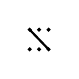
\begin{tikzpicture}[baseline=1pt]
 \draw [fill] (0,0) circle(0.12ex);
 \draw [fill] (0.12,0) circle(0.12ex);
 \draw [fill] (0,0.25) circle(0.12ex);
 \draw [fill] (0.12,0.25) circle(0.12ex);
  \draw [fill] (0.24,0.25) circle(0.12ex);
   \draw [fill] (0.24,0) circle(0.12ex);
 \draw [thick] (0.24,0)--(0.,0.25);
 \end{tikzpicture}
\right)}

\newcommand{\Pnnanan}{{\mathbb P}\left(
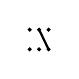
\begin{tikzpicture}[baseline=1pt]
 \draw [fill] (0,0) circle(0.12ex);
 \draw [fill] (0.12,0) circle(0.12ex);
 \draw [fill] (0,0.25) circle(0.12ex);
 \draw [fill] (0.12,0.25) circle(0.12ex);
  \draw [fill] (0.24,0.25) circle(0.12ex);
   \draw [fill] (0.24,0) circle(0.12ex);
 \draw [thick] (0.24,0)--(0.12,0.25);
 \end{tikzpicture}
\right)}

\newcommand{\Pnnanna}{{\mathbb P}\left(
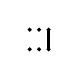
\begin{tikzpicture}[baseline=1pt]
 \draw [fill] (0,0) circle(0.12ex);
 \draw [fill] (0.12,0) circle(0.12ex);
 \draw [fill] (0,0.25) circle(0.12ex);
 \draw [fill] (0.12,0.25) circle(0.12ex);
  \draw [fill] (0.24,0.25) circle(0.12ex);
   \draw [fill] (0.24,0) circle(0.12ex);
 \draw [thick] (0.24,0)--(0.24,0.25);
 \end{tikzpicture}
\right)}






\newcommand{\Pnbc}{{\mathbb P}\left(
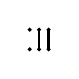
\begin{tikzpicture}[baseline=1pt]
 \draw [fill] (0,0) circle(0.12ex);
 \draw [fill] (0.12,0) circle(0.12ex);
 \draw [fill] (0,0.25) circle(0.12ex);
 \draw [fill] (0.12,0.25) circle(0.12ex);
  \draw [fill] (0.24,0.25) circle(0.12ex);
   \draw [fill] (0.24,0) circle(0.12ex);
 \draw [thick] (0.12,0)--(0.12,0.25);
  \draw [thick] (0.24,0.)--(0.24,0.25);
 \end{tikzpicture}
\right)}

\newcommand{\Pban}{{\mathbb P}\left(
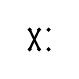
\begin{tikzpicture}[baseline=1pt]
 \draw [fill] (0,0) circle(0.12ex);
 \draw [fill] (0.12,0) circle(0.12ex);
 \draw [fill] (0,0.25) circle(0.12ex);
 \draw [fill] (0.12,0.25) circle(0.12ex);
  \draw [fill] (0.24,0.25) circle(0.12ex);
   \draw [fill] (0.24,0) circle(0.12ex);
 \draw [thick] (0.0,0)--(0.12,0.25);
  \draw [thick] (0.12,0.)--(0.,0.25);
 \end{tikzpicture}
\right)}

\newcommand{\Pncb}{{\mathbb P}\left(
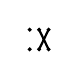
\begin{tikzpicture}[baseline=1pt]
 \draw [fill] (0,0) circle(0.12ex);
 \draw [fill] (0.12,0) circle(0.12ex);
 \draw [fill] (0,0.25) circle(0.12ex);
 \draw [fill] (0.12,0.25) circle(0.12ex);
  \draw [fill] (0.24,0.25) circle(0.12ex);
   \draw [fill] (0.24,0) circle(0.12ex);
 \draw [thick] (0.24,0)--(0.12,0.25);
  \draw [thick] (0.12,0.)--(0.24,0.25);
 \end{tikzpicture}
\right)}

\newcommand{\Pbcn}{{\mathbb P}\left(
\begin{tikzpicture}[baseline=1pt]
 \draw [fill] (0,0) circle(0.12ex);
 \draw [fill] (0.12,0) circle(0.12ex);
 \draw [fill] (0,0.25) circle(0.12ex);
 \draw [fill] (0.12,0.25) circle(0.12ex);
  \draw [fill] (0.24,0.25) circle(0.12ex);
   \draw [fill] (0.24,0) circle(0.12ex);
 \draw [thick] (0.0,0)--(0.12,0.25);
  \draw [thick] (0.12,0.)--(0.24,0.25);
 \end{tikzpicture}
\right)}

\newcommand{\Pnab}{{\mathbb P}\left(
\begin{tikzpicture}[baseline=1pt]
 \draw [fill] (0,0) circle(0.12ex);
 \draw [fill] (0.12,0) circle(0.12ex);
 \draw [fill] (0,0.25) circle(0.12ex);
 \draw [fill] (0.12,0.25) circle(0.12ex);
  \draw [fill] (0.24,0.25) circle(0.12ex);
   \draw [fill] (0.24,0) circle(0.12ex);
 \draw [thick] (0.24,0)--(0.12,0.25);
  \draw [thick] (0.12,0.)--(0.,0.25);
 \end{tikzpicture}
\right)}

\newcommand{\Pnba}{{\mathbb P}\left(
\begin{tikzpicture}[baseline=1pt]
 \draw [fill] (0,0) circle(0.12ex);
 \draw [fill] (0.12,0) circle(0.12ex);
 \draw [fill] (0,0.25) circle(0.12ex);
 \draw [fill] (0.12,0.25) circle(0.12ex);
  \draw [fill] (0.24,0.25) circle(0.12ex);
   \draw [fill] (0.24,0) circle(0.12ex);
 \draw [thick] (0.24,0)--(0.,0.25);
  \draw [thick] (0.12,0.)--(0.12,0.25);
 \end{tikzpicture}
\right)}

\newcommand{\Pcbn}{{\mathbb P}\left(
\begin{tikzpicture}[baseline=1pt]
 \draw [fill] (0,0) circle(0.12ex);
 \draw [fill] (0.12,0) circle(0.12ex);
 \draw [fill] (0,0.25) circle(0.12ex);
 \draw [fill] (0.12,0.25) circle(0.12ex);
  \draw [fill] (0.24,0.25) circle(0.12ex);
   \draw [fill] (0.24,0) circle(0.12ex);
 \draw [thick] (0.0,0)--(0.24,0.25);
  \draw [thick] (0.12,0.)--(0.12,0.25);
 \end{tikzpicture}
\right)}

